\documentclass{article}
\usepackage{amsmath,amssymb,amsthm,tikz,float,caption,enumitem,algpseudocode,mathtools}
\newtheorem*{thm} {Theorem}
\title{\vspace{-3.5cm}CSC 225 Written Assignment 1}
\author{Oliver Tonnesen}
\date{June 3, 2018}
\begin{document}
\maketitle
	% Beginning part a of question 1
\renewcommand{\thesubsection}{\thesection.\alph{subsection}}
\section{Proofs by Induction}
\subsection{}
	If the shape resulting from the cells shaded during any given step n is considered, a pattern can be observed by breaking the shape into four segments. Steps zero to three will be shown as examples:
	\begin{figure}[H]
		\centering
		\begin{minipage}{.45\textwidth}
			\centering
			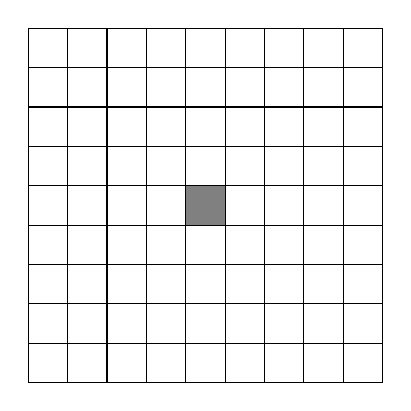
\begin{tikzpicture}[every node/.style={minimum size=.5cm-\pgflinewidth, outer sep=0pt}]
    \draw[step=0.5cm,color=black] (-1,-1) grid (3.5,3.5);
    \node[fill=gray] at (1.25,1.25) {};
\end{tikzpicture}

			%\captionsetup{labelformat=empty}
			\caption{Step 0}
		\end{minipage}\hfill
		\begin{minipage}{.45\textwidth}
			\centering
			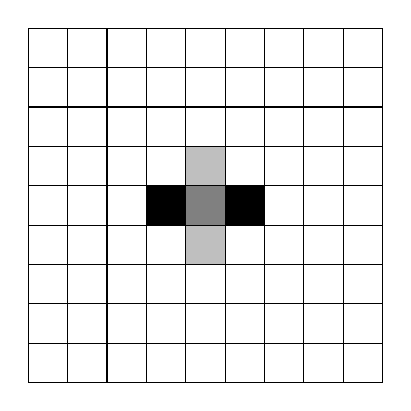
\begin{tikzpicture}[every node/.style={minimum size=.5cm-\pgflinewidth, outer sep=0pt}]
    \draw[step=0.5cm,color=black] (-1,-1) grid (3.5,3.5);
    \node[fill=gray] at (1.25,1.25) {};
    \node[fill=gray!50] at (1.25,1.75) {};
    \node[fill=gray!50] at (1.25,.75) {};
    \node[fill=black!100] at (1.75,1.25) {};
    \node[fill=black!100] at (.75,1.25) {};
\end{tikzpicture}

			%\captionsetup{labelformat=empty}
			\caption{Step 1}
		\end{minipage}\hfill
	\end{figure}
	\begin{figure}[H]
		\centering
		\begin{minipage}{.45\textwidth}
			\centering
			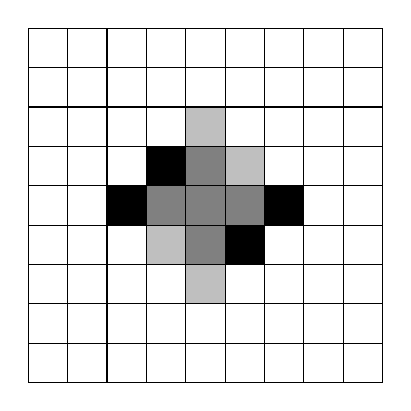
\begin{tikzpicture}[every node/.style={minimum size=.5cm-\pgflinewidth, outer sep=0pt}]
    \draw[step=0.5cm,color=black] (-1,-1) grid (3.5,3.5);
    \node[fill=gray] at (1.25,1.25) {};
    \node[fill=gray] at (1.25,1.75) {};
    \node[fill=gray] at (1.25,.75) {};
    \node[fill=gray] at (1.75,1.25) {};
    \node[fill=gray] at (.75,1.25) {};
    \node[fill=gray] at (1.25,1.25) {};
    \node[fill=gray] at (1.25,1.25) {};
    \node[fill=gray!50] at (1.25,2.25) {};
    \node[fill=gray!50] at (1.25,.25) {};
    \node[fill=black!100] at (2.25,1.25) {};
    \node[fill=black!100] at (.25,1.25) {};
    \node[fill=gray!50] at (1.75,1.75) {};
    \node[fill=gray!50] at (.75,.75) {};
    \node[fill=black!100] at (1.75,.75) {};
    \node[fill=black!100] at (.75,1.75) {};
\end{tikzpicture}

			%\captionsetup{labelformat=empty}
			\caption{Step 2}
		\end{minipage}\hfill
		\begin{minipage}{.45\textwidth}
			\centering
			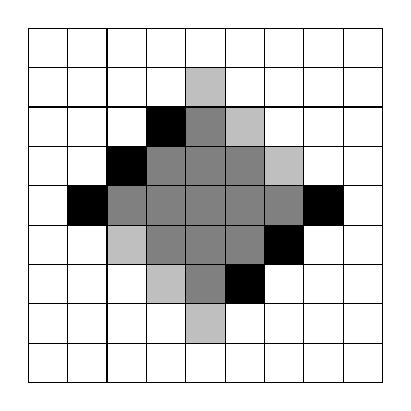
\begin{tikzpicture}[every node/.style={minimum size=.5cm-\pgflinewidth, outer sep=0pt}]
    \draw[step=0.5cm,color=black] (-1,-1) grid (3.5,3.5);
    \node[fill=gray] at (1.25,1.25) {};
    \node[fill=gray] at (1.25,1.75) {};
    \node[fill=gray] at (1.25,.75) {};
    \node[fill=gray] at (1.75,1.25) {};
    \node[fill=gray] at (.75,1.25) {};
    \node[fill=gray] at (1.25,1.25) {};
    \node[fill=gray] at (1.25,1.25) {};
    \node[fill=gray] at (1.25,2.25) {};
    \node[fill=gray] at (1.25,.25) {};
    \node[fill=gray] at (2.25,1.25) {};
    \node[fill=gray] at (.25,1.25) {};
    \node[fill=gray] at (1.75,1.75) {};
    \node[fill=gray] at (.75,.75) {};
    \node[fill=gray] at (1.75,.75) {};
    \node[fill=gray] at (.75,1.75) {};
    \node[fill=gray] at (1.25,1.75) {};
    \node[fill=gray] at (1.25,.75) {};
    \node[fill=gray!50] at (1.25,2.75) {};
    \node[fill=gray!50] at (1.75,2.25) {};
    \node[fill=gray!50] at (2.25,1.75) {};
    \node[fill=black!100] at (2.75,1.25) {};
    \node[fill=black!100] at (2.25,.75) {};
    \node[fill=black!100] at (1.75,.25) {};
    \node[fill=gray!50] at (1.25,-.25) {};
    \node[fill=gray!50] at (.75,.25) {};
    \node[fill=gray!50] at (.25,.75) {};
    \node[fill=black!100] at (-.25,1.25) {};
    \node[fill=black!100] at (.25,1.75) {};
    \node[fill=black!100] at (.75,2.25) {};
\end{tikzpicture}

			%\captionsetup{labelformat=empty}
			\caption{Step 3}
		\end{minipage}\hfill
	\end{figure}
	It can clearly be seen that for any step n, four distinct groups of cells are shaded, each of which containing exactly n cells.
	From this observation can be crafted a simple recurrence relation: 
	\[S_n = 4n + S_{n-1}\]
	Where $S_n$ represents the number of cells shaded in step $n$.
	% Beginning part b of question 1
\subsection{}
	\begin{thm}\ \\
		For any $n \geq 0$, $n \in \mathbb{Z}$, the number of cells shaded in step n is represented by the function
		\begin{align}
			f(n) = 2n^2+2n+1
		\end{align}
	\end{thm}
	\begin{proof}
		As shown in section 1.a, $S_n$ % Replace [the previous section] with a or something
		represents the number of cells shaded in step n. If $f(n)$ can be shown to be equal to $S_n$ for all $n$,
		then $f(n)$ must also represent the number of cells shaded in step n.\\
		\newline
		Claim: $S_n = f(n)$\\\\
		Base case $n=0$:
		\begin{align*}
			S_0 &= f(0)\\
			1 &= 2(0)^2+2(0)+1\\
			1 &= 1
		\end{align*}\\
		Inductive Hypothesis: Suppose the theorem holds for all values of $n$ up to some $k$, $k \geq 0$. Then, $S_n = f(n)$ is true when $n = k$.\\\\
		Inductive Step: We want to show that the claim is true for all n.\\
		\begin{align*}
			S_k &= f(k) && \text{By the inductive hypothesis}\\
			S_k &= 2k^2+2k+1 && \text{Recall (2)}\\
			(4k+4)+S_k &= (4k+4)+2k^2+2k+1\\
			4(k+1)+S_k &= 2k^2+4k+2+2k+2+1\\
			S_{k+1} &= 2(k+1)^2+2(k+1)+1 && \text{Recall (1)}\\
			S_{k+1} &= f(k+1) && \text{Recall (2)}\\
		\end{align*}
		So by induction, the claim holds that $S_n = f(n)$, and therefore the number of cells shaded at step $n$ is $f(n)$.
	\end{proof}
\section{Algorithm Analysis}
	\begin{enumerate}[label=(\alph*)]
		\item $nlog_2{n}$
		\item $2n$
	\end{enumerate}
\section{Algorithm Design}
\subsection{}
	\begin{algorithmic}[1]
		\Function{MostFrequentElement}{n, k, A}
		\State $tmp \gets \textrm{Zero-valued integer array of size k}$
		\For{$i \gets 0, 1, 2, \ldots, n$}
			\State $tmp[A[i]] \gets tmp[A[i]]+1$
		\EndFor
		\State $max \gets 0$
		\For{$i \gets 0, 1, 2, \ldots, k$}
			\If{$tmp[i]>max$}
				\State $max \gets tmp[i]$
			\EndIf
		\EndFor
		\State \Return max
		\EndFunction
	\end{algorithmic}
	The algorithm always runs exactly once through a for loop for $n$ iterations and once for $k$ iterations, thus the worst-case running time is O($n+k$).
	As can be seen on line 8, the value to be returned is only changed if it is strictly greater than its previously greatest value, so the smallest value
	is always returned if multiple elements are tied for the most occurrences.
\subsection{}
	\begin{algorithmic}[1]
		\Function{MostFrequentElement}{n, k, A}
		\State $sort(A)$\Comment{Sort A in $nlog_2{n}$ time}
		\State $count \gets 0$\Comment{Temp var for occurrences of an element}
		\State $max \gets 0$\Comment{Max element occurrences so far}
		\State $maxItem \gets 0$\Comment{Largest element seen so far}
		\State $prev \gets 0$\Comment{Last seen element}
		\For{$i \gets 0, 1, 2, \ldots, n$}
			\If{$A[i]\neq prev$}
				\If{$count>max$}
					\State $max \gets count$
					\State $maxItem \gets prev$
				\EndIf
				\State $prev \gets A[i]$
				\State $count \gets 0$
			\EndIf
			\State $count \gets count+1$
		\EndFor
		\If{$count>max$}\Comment{Check if last item was most the frequent}
			\State \Return prev
		\EndIf
		\State \Return maxItem
		\EndFunction
	\end{algorithmic}
	The for loop from lines 7 to 17 is run once for n iterations. Since an array can always be sorted in at least $nlog_2{n}$ time,
	the worst case running time is O($nlog_2{n}$).
\subsection{}
	Because of the nature of the problem, each element in A must be inspected, thus the running time of any correct algorithm will always be $\Omega(n)$ and can therefore never be $O(log_2{n})$.
\section{Recurrence Relations}
\subsection{}
	$T(n)=2\cdot3^{log_7{n}}+\sum\limits_{i=0}^{log_7{n}-1}3^i(\dfrac{n}{7^{i+1}}+1)$
\subsection{}
	\begin{thm}\ \\
		For all $n > 0$ where $n$ is of the form $n = 7^k$ for some $k \in \mathbb{Z}$:
		\begin{align*}
			T(n) = 2\cdot3^{log_7{n}}+\sum\limits_{i=0}^{log_7{n}-1}3^i(\dfrac{n}{7^{i+1}}+1)
		\end{align*}
	\end{thm}
	\begin{proof}
		Base case $n=1$:
		\begin{align*}
			T(1) &= 2\cdot3^{log_7{1}}+\sum\limits_{i=0}^{log_7{1}-1}3^i(\dfrac{1}{7^{i+1}}+1)\\
			T(1) &= 2\\
			2 &= 2 && \text{$T(1)=2$ by the definition of $T(n)$.}
		\end{align*}
		Let $n=7^k$, then\\
		\[T(n)=T(7^k)\]
		and
		\[2\cdot3^{log_7{n}}+\sum\limits_{i=0}^{log_7{n}-1}3^i(\dfrac{n}{7^{i+1}}+1)=2\cdot3^k+\sum\limits_{i=0}^{k-1}3^i(7^{k-1-i}+1).\]
		Inductive Hypothesis: Suppose there exists some $l$ such that
		\[T(7^k)=2\cdot3^k+\sum\limits_{i=0}^{k-1}3^i(7^{k-1-i}+1).\]
		for all $k \leq l$.\\\\
		Inductive Step: We want to show that the claim is true for all k.
		\begin{align*}
			T(7^k) &= 2\cdot3^k+\sum\limits_{i=0}^{k-1}3^i(7^{k-1-i}+1) && \text{By the inductive hypothesis}\\
			3\cdot T(7^k) &= 3\cdot(2\cdot3^k+\sum\limits_{i=0}^{k-1}3^i(7^{k-1-i}+1))\\
			&= 2\cdot3^{k+1}+3\cdot\sum\limits_{i=0}^{k-1}3^i(7^{k-1-i}+1))\\
			&= 2\cdot3^{k+1}+\sum\limits_{i=0}^{k-1}3^{i+1}(7^{k-1-i}+1))\\
		\end{align*}
		If the sum is expanded out, we get:
		\begin{align*}
			&= 2\cdot3^{k+1}+[3^1(7^{k-1}+1)+3^2(7^{k-2}+1)+\cdots+3^{k-1}(7^0+1)]\\
			\begin{split}
			&= 2\cdot3^{k+1}+[3^1(7^{k-1}+1)+3^2(7^{k-2}+1)+\cdots+3^{k-1}(7^0+1)]\\
			&\qquad+3^0(7^k+1)-3^0(7^k+1)\\
			\end{split}\\
			3\cdot T(7^k)+7^k+1 &= 2\cdot3^{k+1}+[3^0(7^k+1)+3^1(7^{k-1}+1)+\cdots+3^{k-1}(7^0+1)]\\
		\end{align*}
		By the definition of $T(n)$, we have:
		\begin{align*}
			T(7^{k+1}) &= 2\cdot3^{k+1}+[3^0(7^k+1)+3^1(7^{k-1}+1)+3^2(7^{k-2}+1)+\cdots+3^{k-1}(7^0+1)]\\
			&= 2\cdot3^{(k+1)}+\sum\limits_{i=0}^{(k+1)-1}3^i(7^{(k+1)-1-i}+1)\\
			T(7^{k+1}) &= 2\cdot3^{(k+1)}+\sum\limits_{i=0}^{(k+1)-1}3^i(7^{(k+1)-1-i}+1)
		\end{align*}
		So by induction, the hypothesis holds that
		\[T(7^k)=2\cdot3^k+\sum\limits_{i=0}^{k-1}3^i(7^{k-1-i}+1).\]
		Since we defined $n=7^k$, it also holds that
		\[T(n)=2\cdot3^{log_7{n}}+\sum\limits_{i=0}^{log_7{n}-1}3^i(\dfrac{n}{7^{i+1}}+1).\]
	\end{proof}
\end{document}
